
\documentclass{beamer}

\usepackage{booktabs}
\usepackage{graphicx}
\usepackage{multirow}
\usepackage{tabularx}
\usepackage[british]{datetime2}
\usetheme{default}
\usecolortheme{seagull}
\usepackage{newtxtext}
\setbeamertemplate{navigation symbols}{} % No navigation symbols
\setbeamercovered{transparent}

\setbeamertemplate{itemize item}{\color{white}$\bullet$} 
% Include above line to remove bullet indicators

\setbeamertemplate{footline}{
\begin{tabularx}{\textwidth} {
	 >{\raggedright\arraybackslash}X 
  	 >{\centering\arraybackslash}X 
  	 >{\centering\arraybackslash}X 
  	 >{\centering\arraybackslash}X 
  	 >{\centering\arraybackslash}X 
  	 >{\centering\arraybackslash}X}
	
	\insertshortauthor & 
	\insertshorttitle &
	\insertdate &
	\insertsection &
	$\big|$ \insertframenumber /\inserttotalframenumber
\end{tabularx}
}

\makeatletter
\makeatother

%----------------------------------------------------------------------------------------
%	TITLE PAGE
%----------------------------------------------------------------------------------------

\title[Trial Lecture]{The Effects of Slavery and Colonialism on Contemporary
African Politics}

\subtitle{Trial Lecture}

\author[Wishman]{Marius Swane Wishman} 
\date{\today} 
\institute{NTNU}

\begin{document}

\begin{frame}[plain]
\titlepage 
\end{frame}

\section{Introduction} 

\begin{frame}{This lecture will cover}
\begin{itemize}
	\item The slave trade 
\begin{itemize}
	\item[-] Scope and effects 
\end{itemize}
	\item Colonialism 
		\begin{itemize}
			\item[-] Effects on the number of states 
			\item[-] Local and national level effects 
			
		\end{itemize}
	\item Outcomes (dependent variables)
		\begin{itemize}
			\item[-] Conflict
			\item[-] Economic development
			\item[-] Democracy
		\end{itemize}
\end{itemize}	
\end{frame}

\begin{frame}{Conflict}
\begin{figure}
	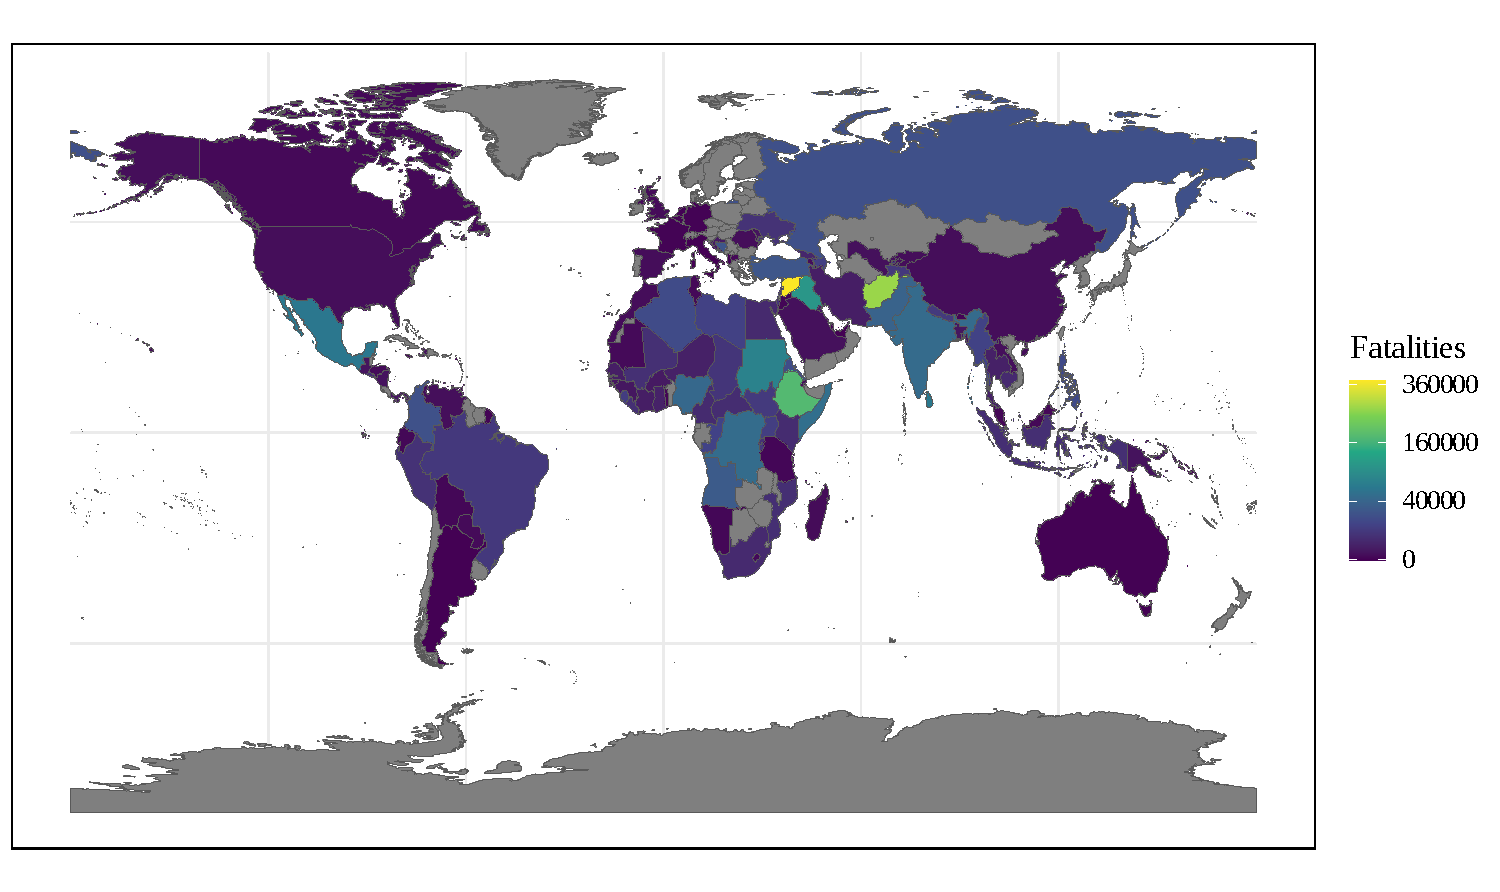
\includegraphics[width=\linewidth]{img/gedplot.pdf}
\end{figure}	
\end{frame}

\begin{frame}{Economic development}
	\begin{figure}
		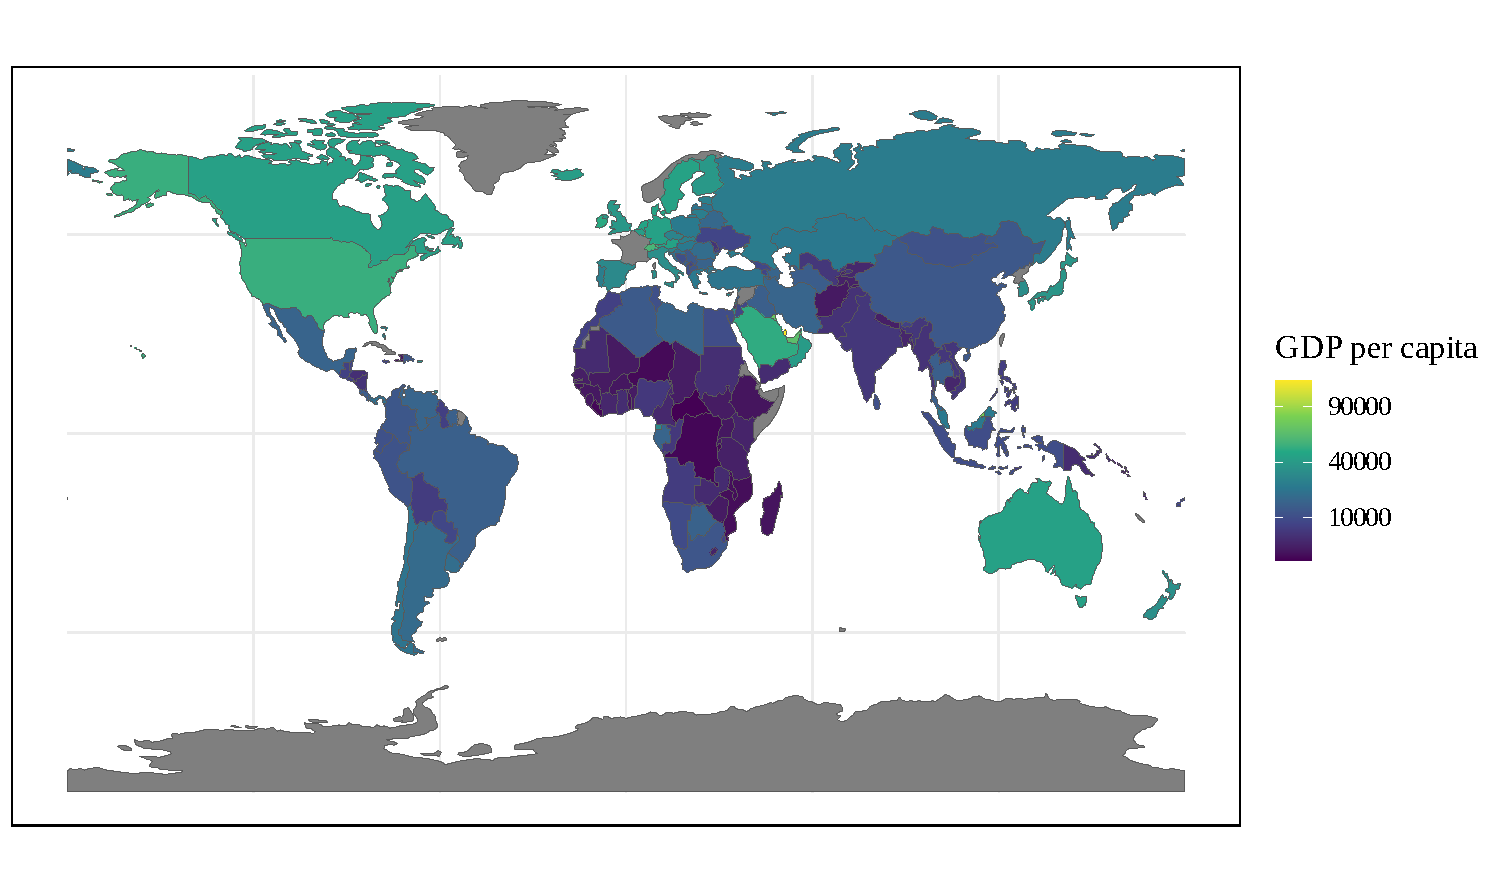
\includegraphics[width=\linewidth]{img/gdpplot.pdf}
	\end{figure}
\end{frame}

\begin{frame}{Democracy}
	\begin{figure} 
		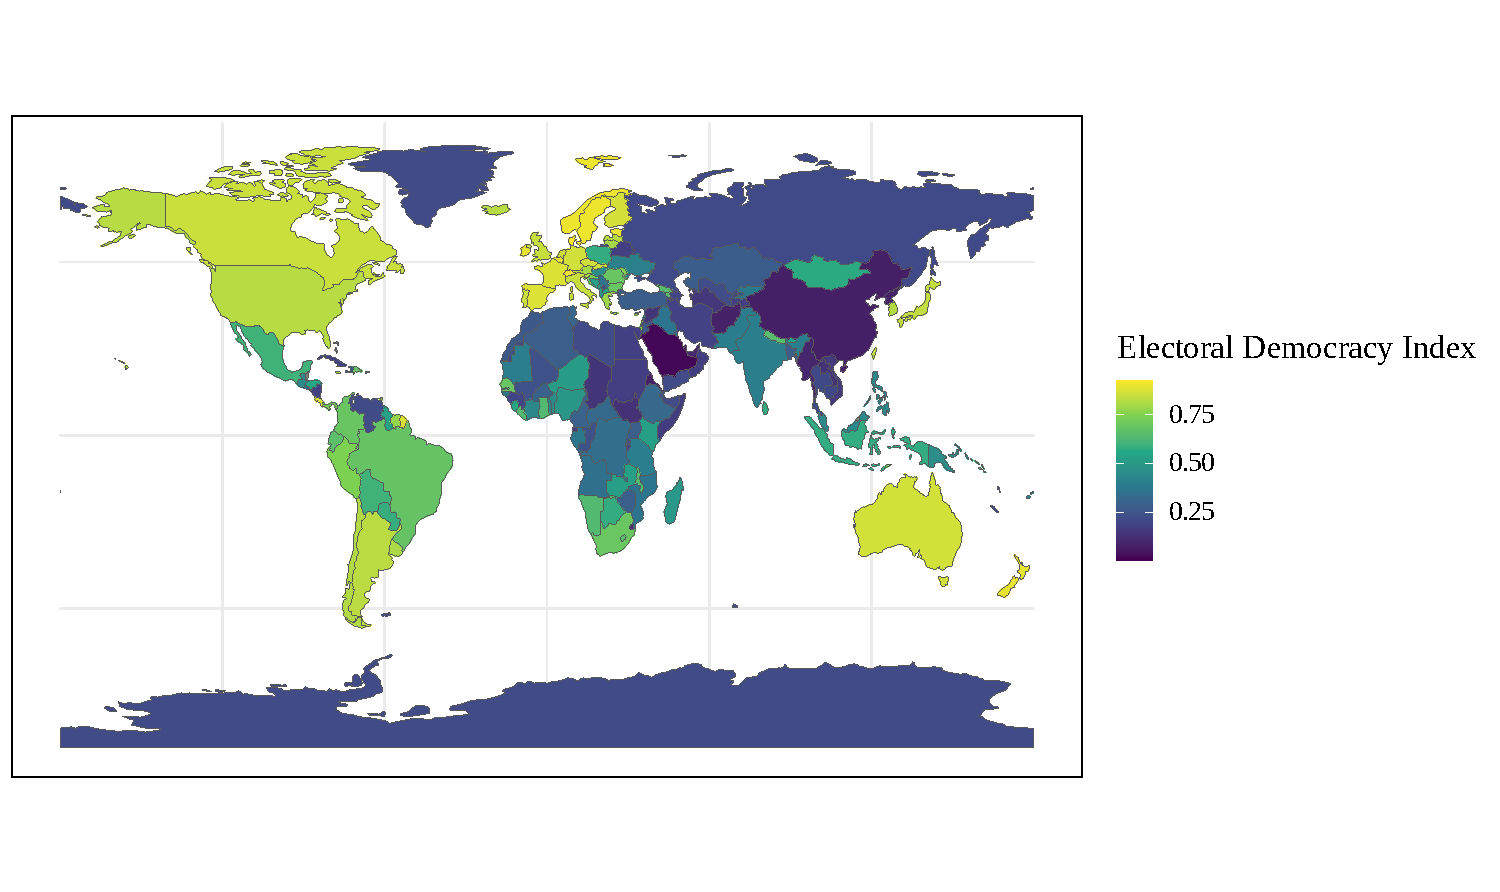
\includegraphics[width=\linewidth]{img/vdemplot.pdf}
	\end{figure}
\end{frame}

\section{The Slave Trade}

\begin{frame}{The African slave trade(s)}

\begin{figure}
	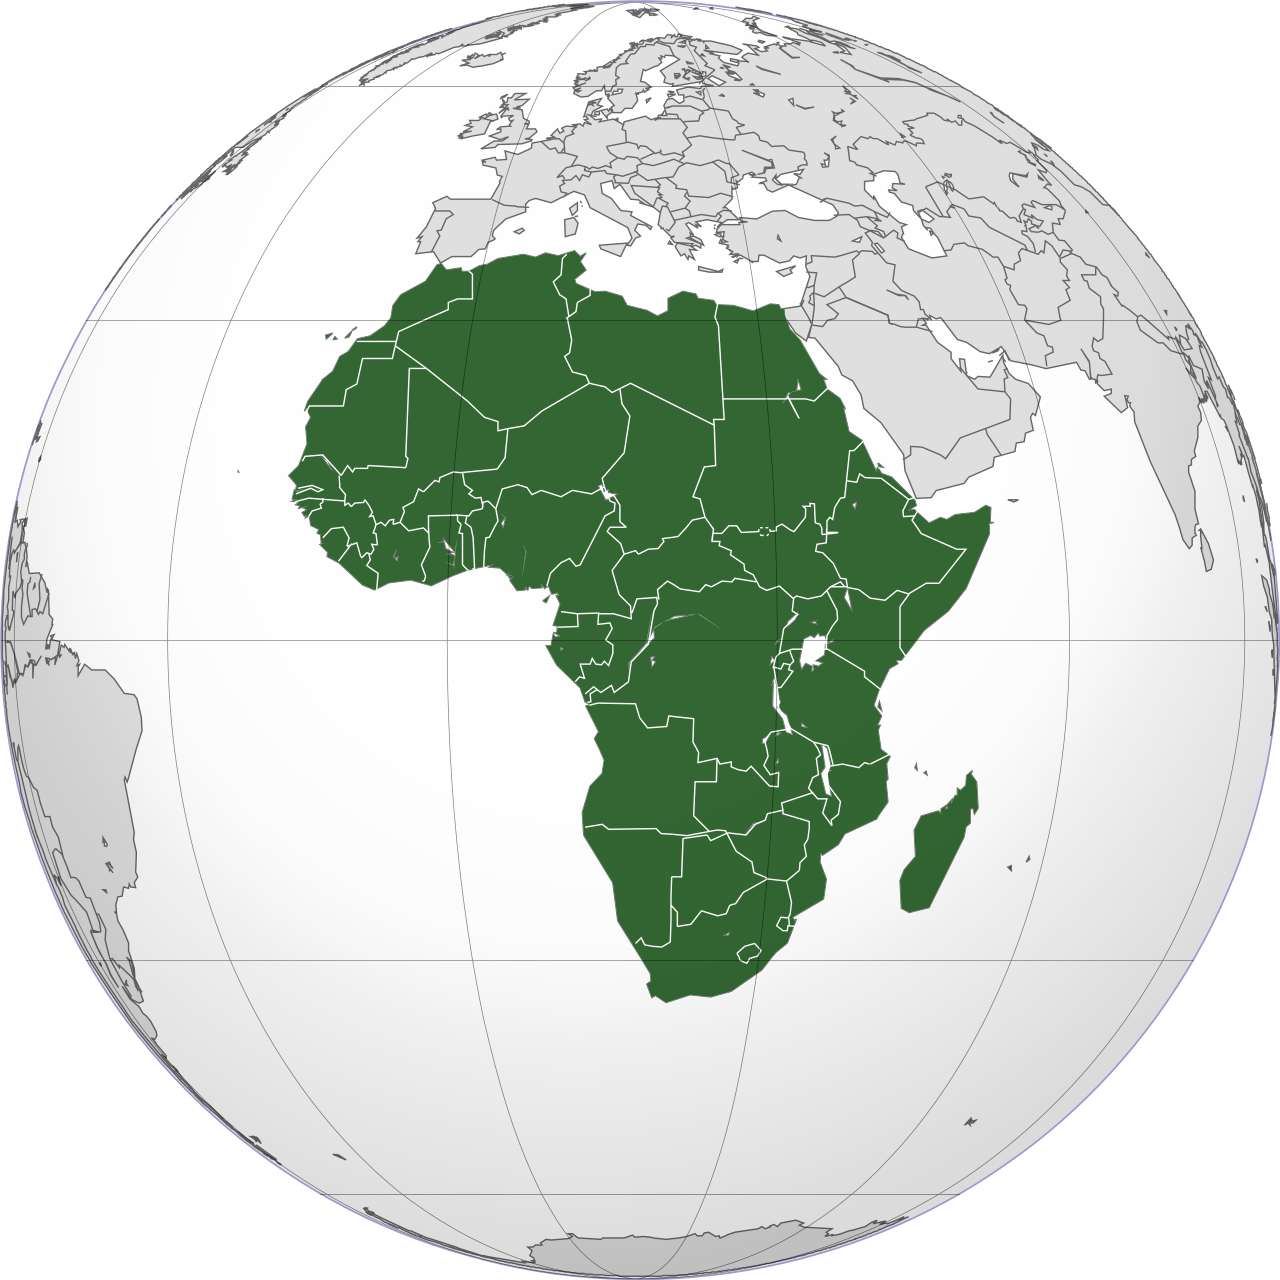
\includegraphics[width=.7\linewidth]{img/africa.png}
\end{figure}

\end{frame}

\section{Colonialism}

\begin{frame}{Colonialism}
	\begin{figure}
		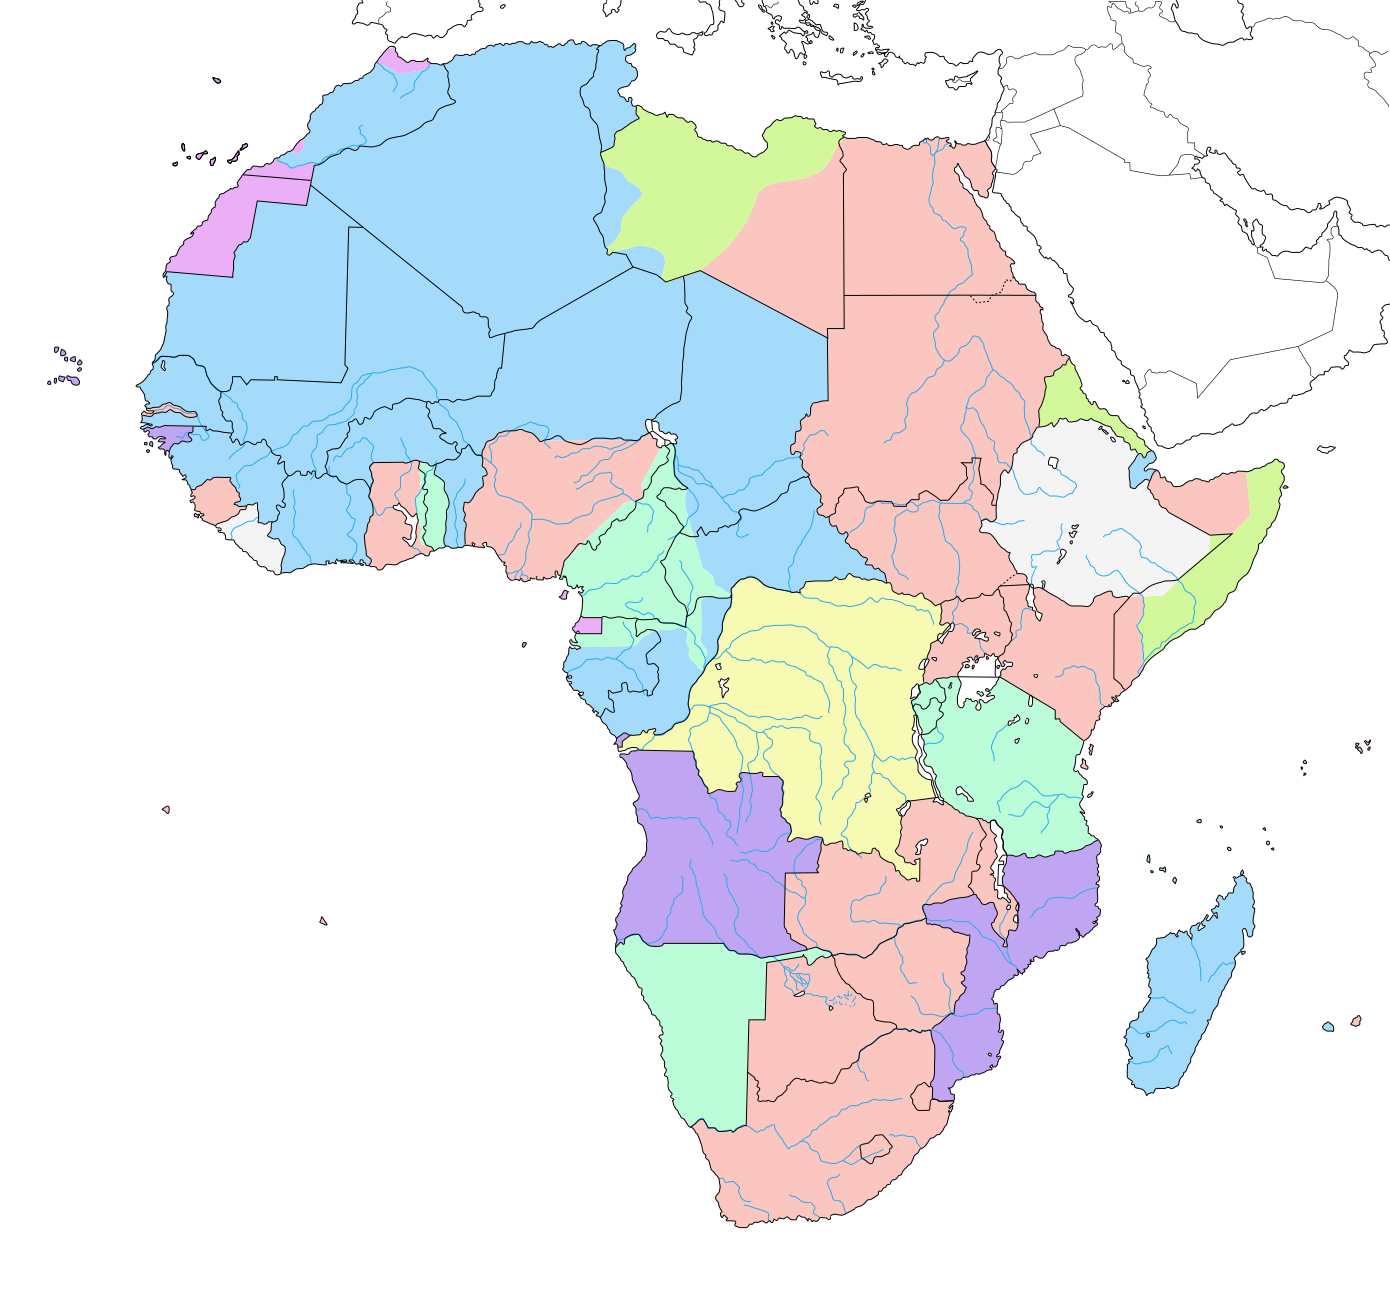
\includegraphics[width=.7\linewidth]{img/colonialAfrica.png}
	\end{figure}
\end{frame}

\begin{frame}
	\begin{figure}
		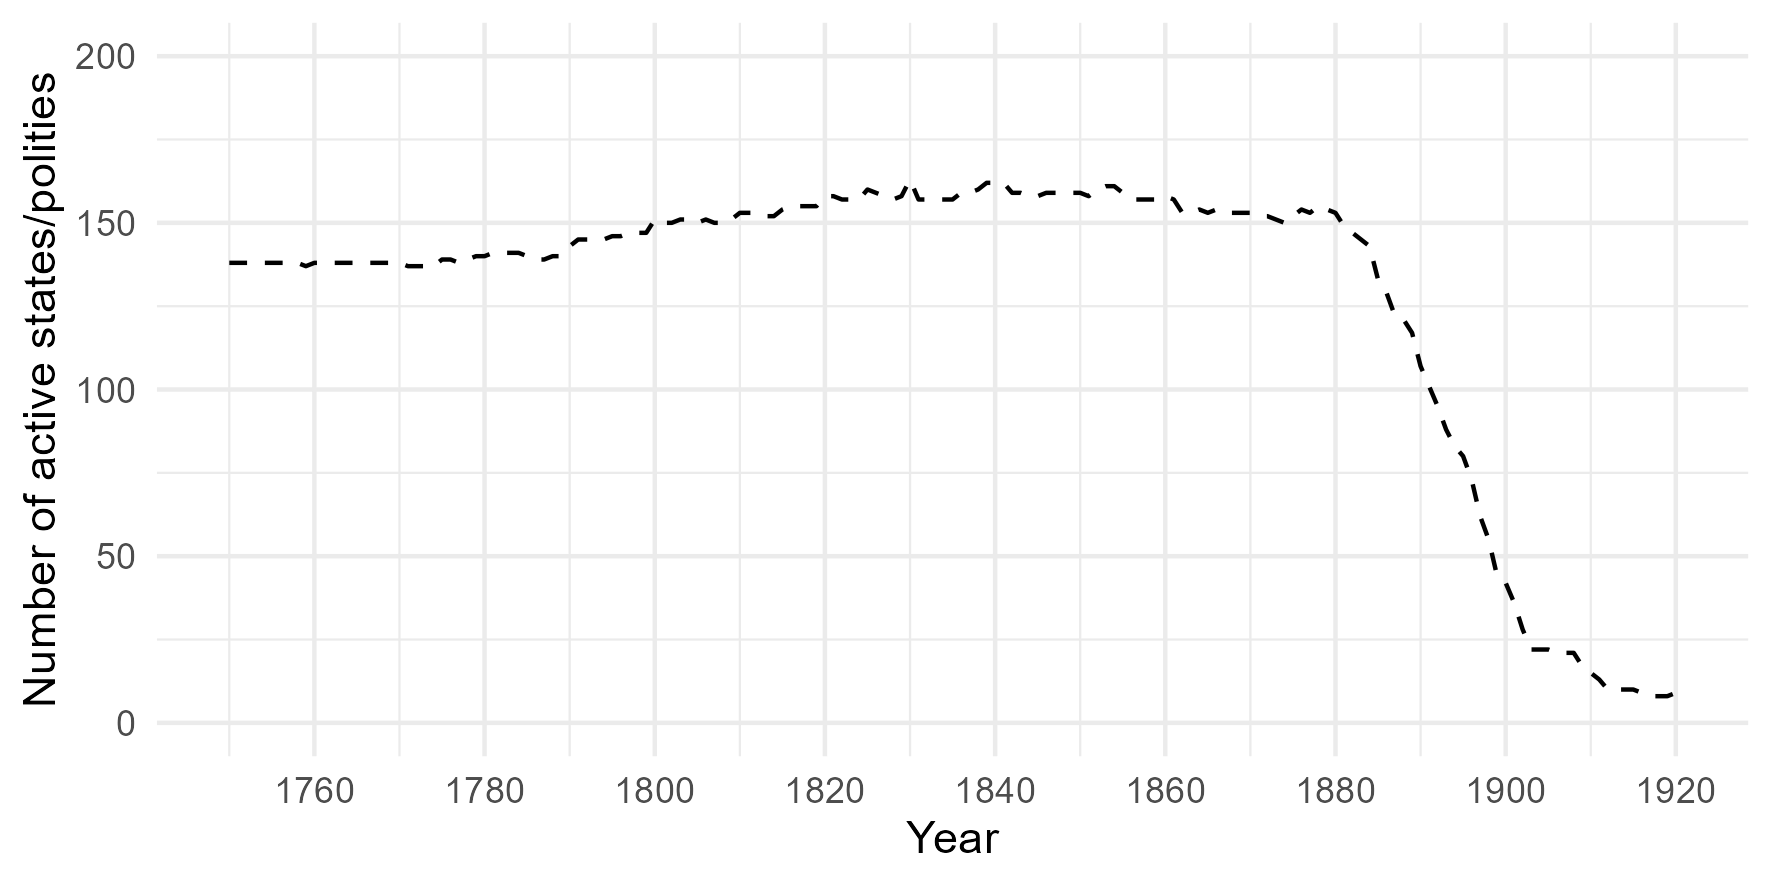
\includegraphics[width=\linewidth]{img/N_States_Only_Over_Time.png}
	\end{figure}
\end{frame}

\begin{frame}
	\begin{figure}
		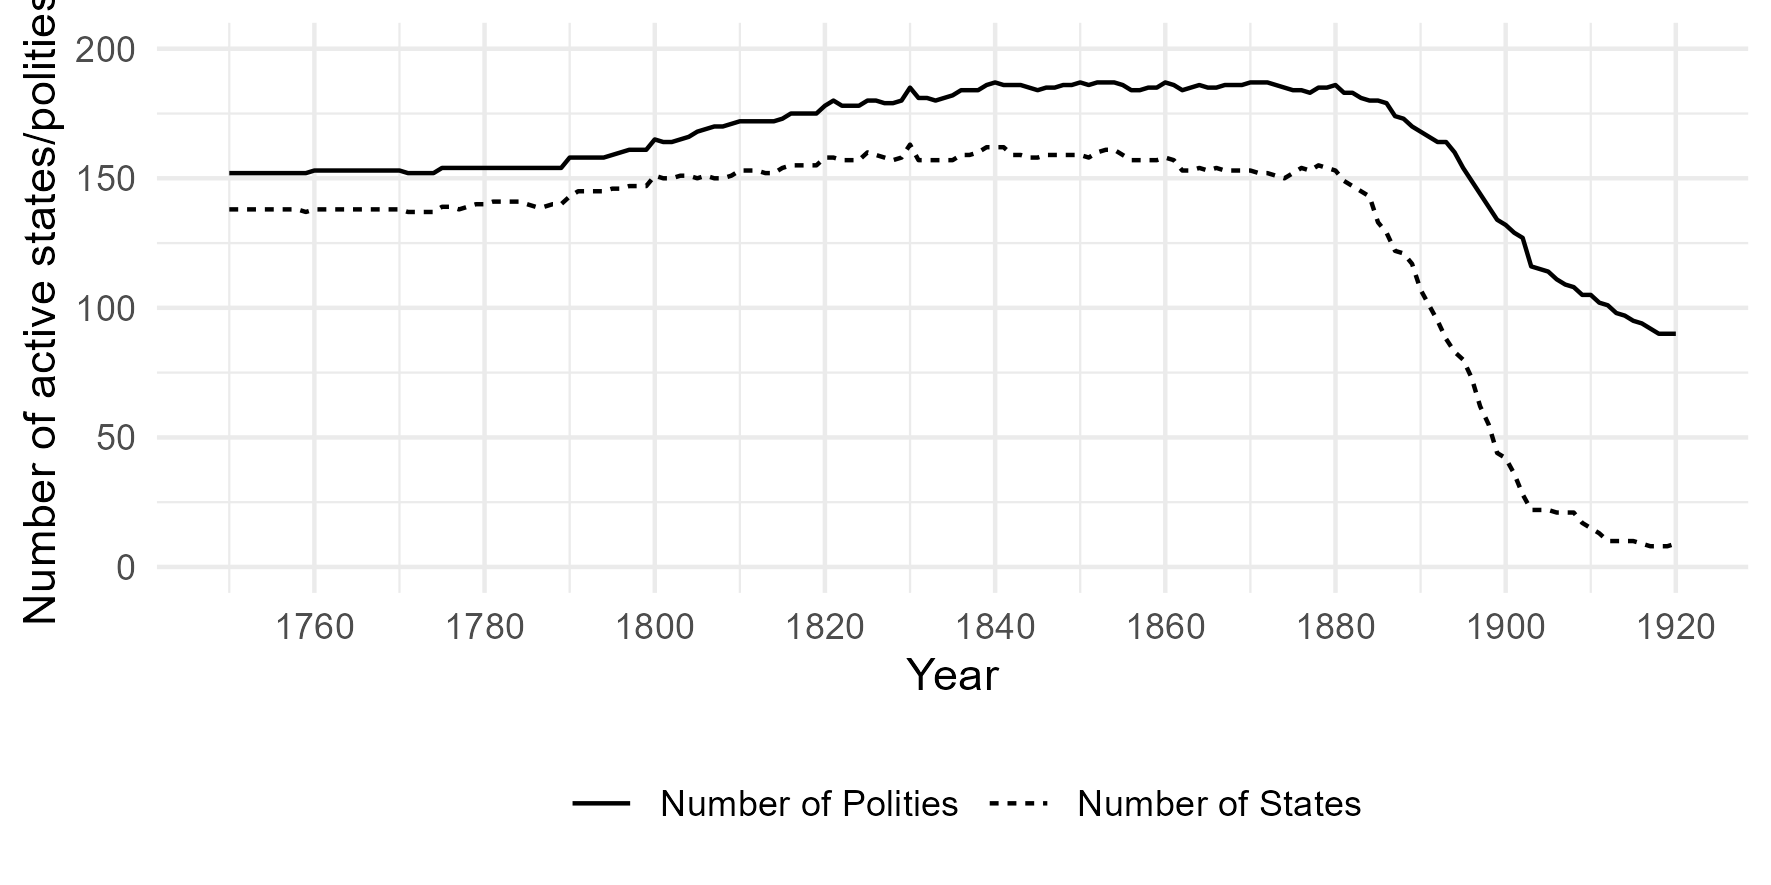
\includegraphics[width=\textwidth]{img/N_States_Over_Time.png}
	\end{figure}
\end{frame}

\section{Conclusion}

\begin{frame}{Conclusion}
	\begin{table}
	\footnotesize	
	\begin{tabularx}{\textwidth}{>{\centering\arraybackslash}X>{\centering\arraybackslash}X>{\centering\arraybackslash}X}
		\toprule
		\multirow{12}{=}{\centering\textbf{The slave trade}} 
					 & \multirow{3}{=}{Ethnic fractionalization} & Conflict \\
					 \cmidrule{3-3}
					 & & Lower contemporary economic development \\	
					 \cmidrule{2-3}
					 & Lower historical and contemporary political development (with
		some exceptions) & Lower contemporary economic development \\
					 \cmidrule{2-3}
				 & \multirow{2}{=}{Lasting enmities between ethnic groups} &
				 Conflict \\
				 \cmidrule{3-3}
				 & & Group based politics \\
		\midrule
		\multirow{5}{=}{\centering\textbf{Colonialism}}
				     & Conflict & \\
			\cmidrule{2-2}
			& Lower contemporary economic development & \\
			\cmidrule{2-2}
			& Democracy (demand for/seeds of) \\
		\bottomrule
	\end{tabularx}
	\end{table}
\end{frame}

\end{document}
